% repeat results and answers in shortened form
\chapter{Conclusion}
\label{chap:conclusion}

% In this study we described the design, creation and evaluation of GeoFront, a web-based point-cloud processing tool.
% Overall, the study has succeeded in what it set out to do: designing and implementing a geo-web-vpl. 
% Moreover, it has delivered a workflow which can be used to quickly configure existing, native geoprocessing libraries written in C++ or Rust to be consumed and used by said geo-web-vpl.  

% This study concludes that based on these measurements, browser-based geo-computation is fast enough that it can enable 
% many promising use-cases, such as on-demand geodata processing apps, educational demo apps, and code sharing. 
% However, extensive user-group testing is required before any definitive statements on accessibility and fitness for geo-computation can be made.  

This chapter contains the conclusion of this study. 
It starts out by answering the research questions posed in the introduction (\refsec{sec:conclusion}), followed up by a summary of the most significant contributions (\refsec{sec:contribution}) and the limitations of these contributions (\refsec{sec:limitations}).
It continues by addressing points of discussion about this study (\refsec{sec:discussion}), which is followed by a number of theorized implications of this study (\refsec{sec:future-work}), a reflection on the value and quality of this study
(\refsec{sec:reflection}), and, lastly, a personal reflection (\refsec{sec:personal-reflection})

% \begin{note}
%   Important: 
%   - Show what I have learned
%   - Show maturity
%   - Recommendations 
%   - Show balance
%   - Show finality
% \end{note}

%%%%%%%%%%%%%%%%%%%%%%%%%%%%%%%%%%%%%%%%%%%%%%%%%%%%%%%%%%%%%%%%%%%%%%%%%%%%%%%
%%%%%%%%%%%%%%%%%%%%%%%%%%%%%%%%%%%%%%%%%%%%%%%%%%%%%%%%%%%%%%%%%%%%%%%%%%%%%%%
%%%%%%%%%%%%%%%%%%%%%%%%%%%%%%%%%%%%%%%%%%%%%%%%%%%%%%%%%%%%%%%%%%%%%%%%%%%%%%%

\section{Conclusion}
\label{sec:conclusion}

This section answers the research questions. 
It starts with answering the sub research questions, and concludes with the answer to the main research question.

\subsection*{Sub Questions}

\begin{itemize}[ ]
  \item 1. "\mySubRQOne"
\end{itemize}

The full answer of this question is represented by \refsec{sec:method:base-vpl} and \refsec{sec:implementation:app}.
Overall, the browser appears to be capable of representing a dataflow-type vpl graph to an acceptable degree, 
based on the implementation presented in \refsec{sec:implementation:app}.
The browsers biggest advantage for an application like this is the amount of features a javascript program can use by default, like the 2D canvas api, the DOM, and WebGL. 
These features do not need to be included within the source code of the application, leading to quick load times. 
All three of these features proved to be vital, and were performant enough to support an application like this. 
Only the 2D canvas Api can become slow when rendering a great number of components. 

TypeScript (JavaScript) was used to represent the data structure and logic needed to make a VPL functional. 
Javascript's flexibility proved to be useful to support features like dynamically loading and using libraries at runtime. 
However, TypeScript's limited type support at runtime, the absence of explicit immutability, and the limited precision in general (no integer atomic, only \m{number}), all hindered the implementation of the VPL model proposed.   

% While the language does offers powerful options for reflection, this cannot truly be used if javascript itself makes no meaningful distinction between number types (\m{int, float, double}), for example.

\begin{itemize}[ ]
  \item 2. "\mySubRQTwo"
\end{itemize}

% To what extent can geocomputation libraries written in system-level languages be compiled
% for web consumption?

Based on the experiments and analysis in \refsec{sec:testing:compilation}, the study concludes that most contemporary, C++-based geocomputation libraries cannot be sufficiently compiled for web consumption, at least not for the purposes of loading the functionalities within a web-VPL.    
This is not due to wasm itself, but rather because of the focus of the emscripten compiler, combined with the implementation requirements of a  web VPL.
Emscripten can be used to compile full-scale C++ applications, and offers an emulation of a POSIX environment.
However, it lacks support for compiling libraries themselves, compared to other wasm-library compilers.
libraries generated with emscripten's 'embind' tool use irregular syntax, which troubles its ability to be loaded programmatically.
While web implementations do exist like 'GDAL-js', these solutions are required to work though Web Workers, and use the emscripten virtual file systems, which again compromises their usage for the purpose of a dataflow-type vpl requiring pure functions.
Finally, the study was able to recognize some discrepancies between the novelty of the WebAssembly format, juxtaposed to 50-year-old legacy of the C++ language, leading to large wasm binaries.

Despite this, the study was able to provide a solution to these compilation shortcomings by expanding the range of 'system-level languages' beyond C++. 
The Rust programming language offers a performance and level of control similar to C++, and has better wasm-library support thanks to the \m{wasm-bindgen} toolkit. 
Using this toolkit, the study could successfully expose a native geocomputation library in a manner properly consumable by a web-vpl.
regrettably, not many rust-based geocomputation libraries are written in pure rust, and the general pool of existing geocomputation libraries is limited due to the novelty of the language. 

Thus, the conclusion is a dilemma between Rust and C++.
C++ has a strong foundation of existing geocomputation libraries compared to newer languages like Rust.  
However, this same legacy inhibits its portability, which makes it harder to compile to web browsers. 
Rust is for the forseeable future a better choice for writing easily consumable, portable libraries, but does not have a fully mature ecosystem of geocomputation libraries yet. 

To offer a solution, the study suggests that either the 'embind' tool must be expanded to the level of functionality of 'wasm-bindgen', or geocomputation libraries must be rewritten in Rust. 
This second option seems counterproductive, but as stated by \citet{ammann_maplibre-rs_2022}: "innovation often requires selectively ignoring prior work."

\begin{itemize}[ ]
  \item 3. "\mySubRQThree"
\end{itemize}

Based on the method described in \refsec{sec:method:plugin-system} and \refsec{sec:implementation:loading}, and the analysis of \refsec{sec:testing:compilation}, it can be concluded that it is possible and even sufficiently usable to load a web-library into a VPL without explicit configuration. 
It also had the desired effect of breaking down the barrier between vpl libraries and regular text-based libraries: Using this method, only one type of library is needed to serve both. 
Moreover, it led to a workflow in which rapid experimentation was possible, since this method allows users to develop a library locally, and then quickly experiment and test its usage online. 

The drawback of allowing this seamless interoperability and rapid experimentation, is that many important properties like descriptions and library metadata do not need to be explicitly specified, and could not be automatically extracted. 
These properties still had to be added to the libraries in the shape of methods with a recognizable naming convention.

Additionally, the freedom of granted by not restricting input and output types can lead to a confusing user experience, since there is no way of restricting libraries to use particular type convention.
Even worse, the libraries could use references pointing to the same object, eliminating the 'immutable, no side effects' nature of a dataflow-type VPL.

\begin{itemize}[ ]
  \item 4. "\mySubRQFour"
\end{itemize}
% To what extent can a 'geo-web-vpl' be \textbf{used} to create geodata pipelines?

Based on the analysis of Geofront in \refsec{sec:testing:usability}, it can be concluded that a geo-web-VPL can be used for geocomputation to a sufficient extent.  
The analysis shows that many of Geofront's best aspects for the purpose of geocomputation are a consequence of the design decision to use a diagram-based, dataflow-type VPL.
Examples of these are how the Functional programming paradigm leads to pure functions and immutable variables, making the graph as a whole behave in a predicable manner, allowing for the inspection of in-between data at runtime. 
However, the openness of the plugin system inhibits the consistency of these functional aspects.
Imported libraries are not forced to exclusively use pure function. 
As a consequence, libraries can create functions with many side effects, or they can use inconsistent input and output datatypes, ultimately leading to confusion for the end-user.

\subsection*{Main Question}

\begin{itemize}[ ]
    \item "\myMainRQ"
\end{itemize}

% How can a VPL be used to support and execute existing geo-computation libraries in a browser?
% So, Does Geofront succeed in "converting existing geocomputation libraries to a sharable VPL format?" 

A VPL can support existing geocomputation libraries if and only if these libraries are able to be \emph{compiled}, \emph{loaded}, and \emph{utilized} in a dataflow VPL format.

Using a new javascript implementation of an acyclic, graph-based VPL, the study was able to demonstrate how the web platform can be used to represent a dataflow-VPL capable of hosting these libraries.
The dataflow-properties of a graph-based VPL like this also makes this libraries sufficiently \emph{usable}, albeit with some well-known caveats of dataflow-VPLS, like the representation of conditionals and iteration. 

The current methods of \emph{compiling} existing C++ geocomputation libraries to the web turned out to be insufficient for the purposes of this study.  
This is due to emscripten's focus on compiling full C++ applications instead of libraries.
Despite this, the study wás able to demonstrate how a novel method can be used to  \emph{compile} and \emph{load} a Rust-library for usage in the VPL.
While not many contemporary geocomputation libraries are written in Rust, the study offers this method to either offer emscripten contributors a blueprint of a desired workflow, or to offer geocomputation library contributors a powerful use-case for the Rust language. 

All in all, this means that either if the Rust ecosystem gains more mature geocomputation libraries, or if Emscripten's capabilities improve, then the code portability problem \& dataflow problem of existing web-based geocomputation VPLS can be overcome. 

%%%%%%%%%%%%%%%%%%%%%%%%%%%%%%%%%%%%%%%%%%%%%%%%%%%%%%%%%%%%%%%%%%%%%%%%%%%%%%%
%%%%%%%%%%%%%%%%%%%%%%%%%%%%%%%%%%%%%%%%%%%%%%%%%%%%%%%%%%%%%%%%%%%%%%%%%%%%%%%
%%%%%%%%%%%%%%%%%%%%%%%%%%%%%%%%%%%%%%%%%%%%%%%%%%%%%%%%%%%%%%%%%%%%%%%%%%%%%%%
%%%%%%%%%%%%%%%%%%%%%%%%%%%%%%%%%%%%%%%%%%%%%%%%%%%%%%%%%%%%%%%%%%%%%%%%%%%%%%%
%%%%%%%%%%%%%%%%%%%%%%%%%%%%%%%%%%%%%%%%%%%%%%%%%%%%%%%%%%%%%%%%%%%%%%%%%%%%%%%
%%%%%%%%%%%%%%%%%%%%%%%%%%%%%%%%%%%%%%%%%%%%%%%%%%%%%%%%%%%%%%%%%%%%%%%%%%%%%%%
%%%%%%%%%%%%%%%%%%%%%%%%%%%%%%%%%%%%%%%%%%%%%%%%%%%%%%%%%%%%%%%%%%%%%%%%%%%%%%%
%%%%%%%%%%%%%%%%%%%%%%%%%%%%%%%%%%%%%%%%%%%%%%%%%%%%%%%%%%%%%%%%%%%%%%%%%%%%%%%
%%%%%%%%%%%%%%%%%%%%%%%%%%%%%%%%%%%%%%%%%%%%%%%%%%%%%%%%%%%%%%%%%%%%%%%%%%%%%%%



\section{Contributions}
\label{sec:contribution}

The study was able to deliver two major contributions:
\begin{itemize}[-]
  \item \textbf{A new implementation of a web-based geocomputation VPL}
    This study introduces a novel javascript implementation of a web-based dataflow-VPL capable of both geometry processing, as well as geocomputation.
    Compared to existing web-based alternatives, this VPL is closer in design and functionality to common geometry VPLs like grasshopper, as it adheres to being a graph-based dataflow VPL. 
% We introduce the \"Geofront\" application, which achieves this accessibility in two ways: 
% Firstly, geoprocessing libraries, written in either Rust or C++, are compiled to WebAssembly: binaries which can be run in any modern browser, client-side. This mitigates the need for any installation, and allows the software to be directly used as soon as a website is fully loaded. WebAssembly offers a performance comparable to native usage. Geofront accepts these binaries as plugins.

% Secondly, Geofront itself is set up as a web-based visual programming environment, complete with a 3D viewer and WMS, WFS \& WMTS support. Using these tools, users can interactively run these geoprocessing libraries with different datasets and parameters. Using visual programming, the user can chain and alter geoprocessing steps, visualize in-between products, and save \& load these workflows.

  \item \textbf{A novel workflow of publishing and using native libraries on the web}
    Secondly, a new workflow was developed to allow a geo-computation function or library to be used within a visual programming environment.
    Moreover, this can be done with a minimum of configuration steps: 
    Any Javascript, Typescript or Rust library which satisfies the conditions layed out in \refsec{sec:implementation:loading:limits}, automatically functions in Geofront.
    
    % CITYJSON VALIDATOR ARGUMENT: THE WEB CAN BE USED TO IMMEDIATELY MAKE SOME TOOL / SOME RESEARCH PROJECT OPERATIONAL 'IN THE REAL WORLD'. THIS WAY, DATA CAN BE GATHERED, USER FEEDBACK CAN BE GATHERED, AND THE TOOL CAN BE EVALUATED IN TERMS OF REPRODUCABILITY. FINALLY, IT OFFERS THE POSSIBILITY OF THE TOOL BEING ACTUALLY USED, IN PRACTICE. 
% z
\end{itemize}

These two contributions together lead to an environment suited for a number of use cases, including: 
\begin{itemize}
  \item Visual debugging: One can use this environment visualize the result of an algorithm in 2D or 3D.
  \item Fine tuning parameters: In situations where algorithms contain unintuitive or empirically derived parameters (e.g. RANSAC), a visual environment can be use to quickly try out multiple settings, and to observe their effects.
  \item Benchmarking: Geofront can be used to test the web performance of multiple algorithms written in different languages. 
  \item Publication: Geofront scripts can be shared using a link. 
    this can be used to make a native library usable online, and by doing so, it may help to lower the delta between 'my library works for me' and 'my library works for someone else'.
\end{itemize} 
The combination of these features together make Geofront unique among both \\ geo-VPLS and web-VPLS. 
by providing the full source code, together will all implementation details given in \refchap{chap:implementation}, this study aims to provide guidance for all subsequent studies on the topic of VPLs, geocomputation, or geoweb applications using WebAssembly.



\section{Limitations}
\label{sec:limitations}

These contributions are bound by following limitations:
\begin{itemize}[-]
  \item \textbf{Only Rust, Js \& Ts library support}
  For now, only libraries written in Rust or Javascript / Typescript can be used in Geofront. 
  Due to the results layed out in \refsec{sec:testing:compilation}, a stable method of using any C++ library can not be provided for at the current moment.

  \item \textbf{In practice, not all libraries can be used }
  \refsec{sec:implementation:loading:limits} shows that not all Rust and JS/TS libraries are supported. 
  Additionally, in order to properly communicate, visualize, and make data interoperable, special 'config' functions and methods are still required. 
  
  \item \textbf{Only small-scale geodata is possible}
  the Geofront environment uses browser-based calculations, which does not lend itself well to process datasets larger than a certain threshold. 
  This means it cannot be used properly for big data, or other expensive processes. 

  % was not part of this study
  % First of all, the purpose of this study was only to get geocomputation libraries to the web, and inside of a vpl format. 
  
  
  % But still, lets give the devil his due:
  % Even when processing "smaller" datasets of, lets say 4 GB, most of the 'flowchart niceties' of geofront will cease to be useful. 
  % Inspecting this data will take more time than its worth, and reconfiguring the flowchart will take a long time. 
  % This can be mitigated by using web workers, but it will still not be very ergonomic to work with. 
  
  % When datasets become larger thansmall datasets of , most of the 'flowchart niceties' of geofront will cease to be useful. 

  \item \textbf{Implementation shortcomings} 
  Geofront is a prototype, and has many usability shortcomings, explained in \refsec{sec:testing:usability}.
  In addition, many geocomputation-specific aspects are missing, such as a topographical base layer.  
\end{itemize}



\section{Discussion}
\label{sec:discussion}
This section covers questions on the decisions made during the study, and the answer this study is able to provide as a response.

\subsubsection*{Q: Geodata is almost always big data. Will this web environment be scalable to handle big datasets?}

% 3. web interface
% - Having no file system really hurts the usefulness of the vpl as a data processing application.
% -> file system API is coming to fix this
% -> This study recommends cloud-native as a solution to this problem, and has added 

% One of the problems to address when considering the ergonomics of geocomputation, is the fact that geodata is almost always big data. 
% A web application cannot be expected to process huge datasets. 
% So how does geofront address this fundamental aspect of geoprocessing? 

The sizeable nature of geodata is a component fundamental to geocomputation.
However, scaling the application up to handle big data deviated too much from the core goal of this thesis to solve the problem of library portability, and had to be left to future work. 

Still, to pose a solution, this study experimented with compiling a \\ full Geofront script to javascript.
This can be regarded as a 'release' build of the Geocomputation pipeline: 
It would have allowed native CLI-execution using Deno \citep{contributors_deno_2022}, without any dependency or reference to Geofront itself.
Only the libraries used within the pipeline would need to be referenced, and this could have been done using regular javascript import statements, and npm.

% While it seems convoluted to compile a native library to WebAssembly and then execute it natively again, it is actually a sound strategy for building scalable, containerized programs for the cloud. 
% The 'WASI' project is a good example of this (Source: https://hacks.mozilla.org/2019/03/standardizing-wasi-a-webassembly-system-interface/). 
However, this experiment turned out to be a full-sized study in itself, and so had to be left to subsequent studies due to time constraints. 

\subsubsection*{Q: Why wasn't Geofront developed as a native application, and published to the web as a whole?}

A native-first build of Geofront would indeed be more performant, especially if the application is fully hybridized:
If both a native and web build of an application are available, then Users can choose for themselves if they wish to sacrifice the performance and native experience for the accessibility of a web build. 
 
However, many features key to the solution and workflow specific to Geofront would be lost in such a setup.  
(Prospected) features like dynamically loading plugins, scriptable components, or the compilation to javascript would be lost, or would have to be regained by incorporating a browser engine \emph{within} this native application. 

However, a valid criticism can be made that this study could have opted for adding more native-first components, such as the maplibre renderer \citep{ammann_maplibre-rs_2022}

% \subsubsection*{Q: Where was this 'barrier' the methodology spoke of?}

% Recall that the methodology states how the barrier preventing geo-web-VPLS from adapting native libraries, 
% must be because of issues encountered during \textbf{compilation}, \textbf{Loading}, \textbf{Representation}, or \textbf{used}, or a combination of these factors. 

% After the conclusion of this study, three major issues can be identified, which indeed occupy spaces in between the above four factors. 

% \textbf{1. Compilation and Loading}

% Firstly, it turned out to be challenging to expose existing libraries in a way usable by a dataflow-vpl. 
% - "just compiling to wasm" was not enough.
% - Webassembly is a double edged sword. Interfacing with wasm binaries from javascript is slow: lots of duplication of data. 
% -> catch 22 beyween rust and C++


% \textbf{2. Disconnect between textual and visual programming}

% Secondly, to turn a 'normal' function into a component usable in a dataflow graph, additional metadata needs to be specified.
% This leads to specific config files and classes, which in turns creates a barrier between regular programming libraries, and vpl libraries. 
% \refsec{sec:implementation:loading} represents the attempted solution to this problem. 


% \textbf{3. Web interfacing}

% And lastly, having limited access to the file system really hurts the usefulness of the vpl as a data processing application.
% This aspect has not been properly addressed during this study.
% This study recommends the novel web services cloud-native as a solution to this problem, and has added 


% \subsubsection*{Q: Is a geo-web-vpl the same as a 3D vpl with existing geoprocessing functionalities attached? In other words, is geoprocessing nothing else than procedural modelling?}

% No, but it is a good start. 
% A geo-web-vpl is \emph{at the very least} a Geometry VPL. 
% Indeed, an actual geocomputation vpl might require more features, such as a global CRS, support of base-maps, more control on precision, etc. 
% These important aspects must be left for future work.

% \subsubsection*{Q: Usage: Who benefits from a web-geo-vpl, and how? }
% This study proposes 4 use-cases:
% \begin{enumerate}[-]
%   \item Educational Sandbox
%   \item Web Demo Environment
%   \item End-user geoprocessing environment 
%   \item Rapid prototyping environment
% \end{enumerate}

% WHY DOES SOMEONE WANT TO TAKE EXISTING LIBRARIES AND TURN THEM INTO A WEB-BASED VPL FORMAT? 
% - interactive, visual debugging 
%   - explaining the behavior of algorithms to yourself and others
%   - why web: collaborative debugging
% - reproducability of results
%   - lowering the delta between "it works for me" and "it works for someone else"
% - improving the 'online presence' of research.
%   - making research results 'usable' via a link
%   - interdisciplinary exchange of ideas


% SO: Geofront is intended as a Computational Geometry Sandbox environment.
% Meant for: 
%  - publication
%  - sharing ideas 
%  - trying things out
%  - debugging code
%  - learning

% NOT for making programming as a whole 'easier'

\subsubsection*{Q: A large reason for developing web-based VPLs is accessibility.  Is this environment accessible?}

This study can only answer this question to a limited degree. 
Based on the analysis given at \refsec{sec:testing:usability}, it is safe to say that based on its features, Geofront is about as accessible as comparable geo-vpls, like Geoflow or Grasshopper. 
However, this analysis is only based on the achieved functionality and features. 
Actual user-testing is required to assess The true accessibility of the tool.

\subsubsection*{Q: Is this environment a competitor to native methods of geocomputation?}

In theory, yes.
Using the workflow as described, native geocomputation libraries could be used on the web at near native performance, without requiring installation.
Additionally, the web offers enough functionality so that even sizable, local datasets could be processed this way.
In practice, the dilemma between Rust and C++ means that in the sort term, this environment will not be used for professional geocomputation.
Additionally, the tool is still in a prototypical state, and will need to be more stable and reliable before being used professionally. 

%%%%%%%%%%%%%%%%%%%%%%%%%%%%%%%%%%%%%%%%%%%%%%%%%%%%%%%%%%%%%%%%%%%%%%%%%%%%%%%
%%%%%%%%%%%%%%%%%%%%%%%%%%%%%%%%%%%%%%%%%%%%%%%%%%%%%%%%%%%%%%%%%%%%%%%%%%%%%%%
%%%%%%%%%%%%%%%%%%%%%%%%%%%%%%%%%%%%%%%%%%%%%%%%%%%%%%%%%%%%%%%%%%%%%%%%%%%%%%%

\section{Future work}
\label{sec:future-work}
The many fields this study draws from mean that a great variety of auxiliary aspects were discovered during the execution ot the study. 
Some of these aspects are listed here, and could lead to interesting topics for follow-up research. 

\subsection{Deployment \& scalability}

\begin{figure}
  \centering
  \graphicspath{ {../../assets/images/implementation/} }
  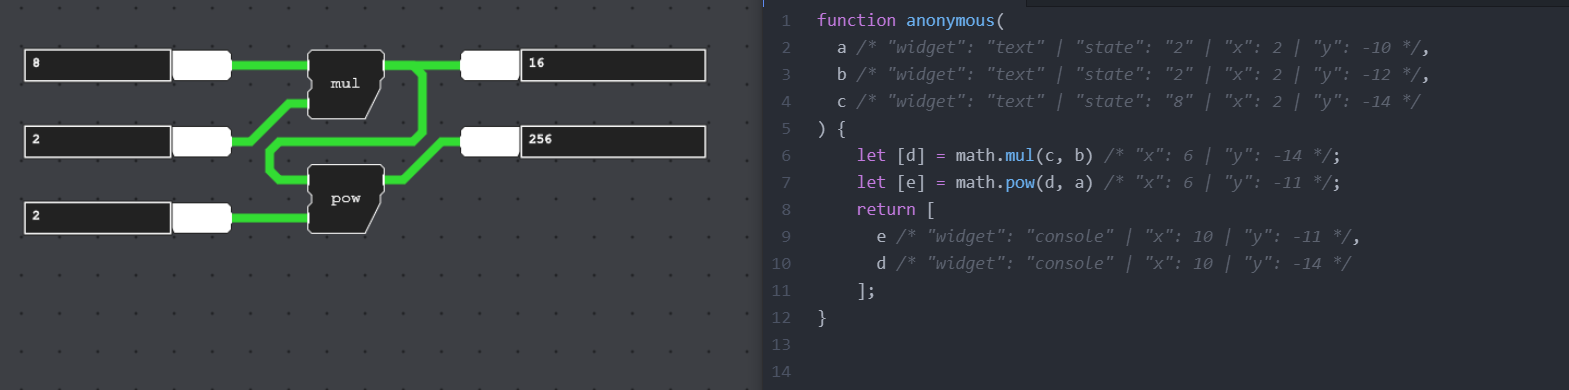
\includegraphics[width=\linewidth]{early-geofront.png}
  \caption[Geofront to js]{An early build of geofront, showing compilation to javascript}
  \label{fig:early-geofront-compile-to-js}
\end{figure}

An early build of Geofront had the ability to compile a Geofront script to regular javascript (see (\reffig{fig:early-geofront-compile-to-js})).  
All libraries were converted to normal import statement, all nodes were replaced by function calls, and the cables substituted by a variable token. 
This way, the application could be run headless (without the \ac{GUI}) either the browser or on a server, using a local javascript runtime like Deno \citep{contributors_deno_2022}.

A future study could re-implement this feature, opening up the possibility for deployment and scalability: 
Scripts created with geofront could then deployed as a web worker, as a web applications of themselves, or as a web processing services \citep{open_geospatial_consortium_web_2015}.
Also, by running this script on a server, and ideally a server containing the geodata required in the process, one could deploy and run a Geofront scripts on a massive scale. 

The overall purpose of this would be to create a \ac{FOSS} alternative to tools like the Google Earth Engine, and FME cloud compute. 

\subsection{Streamed, on demand geocomputation}

This study showed that browser-based geocomputation is reasonably viable. 
This might allow for a new type of geoprocessing workflow, which could replace some use-cases that now require big-data processing and storage.
A big problem in the \ac{GIS} industry is having to process and store sizable datasets, while only a portion of it will be actually used. 
A possible solution could be to take a raw dataset base layer, and process it on-demand in a browser.

This would have several advantages. 
First, end-users can specify the scope and parameters of this process, making the data immediately fine-tuned to the specific needs of this user. 
Secondly, this could be a more cost-effective method, as cloud computation \& Terabytes of storage are time consuming and expensive phenomena.

This type of \emph{on demand geocomputation} is certainly not a drop-in replacement for all use cases. 
But, in situations which can guarantee a 'local correctness', and if the scope asked by the used is not too large, this should be possible. 
Examples of this would be a streamed delaunay triangulation, TIN interpolation or color-band arithmetic. 

\subsection{Rust-based geocomputation \& cloud native geospatial}

An interesting aspect this study was able to touch on is using Rust for geocomputation.
The reason for this was the extensive support for webassembly, which was essential for browser-based geocomputation. 
However, there are additional reasons one might want to perform geocomputation within Rust.
One is that rust is widely considered as a more stable, less runtime error-prone language than C++, while offering similar performance and features.
Additionally, rust Wasm binaries also tend to be smaller than C++ wasm binaries.  

This could be very interesting to the "cloud-native geospatial" movement. 
This \ac{GIS} movement aims to create the tools necessary to send geocomputation to servers, rather than sending geodata to the places where they are processed.
To do this, geocomputation must become much more portable than it currently is, and Rust compiled to WebAssembly might proof to be a strong candidate for creating exchangeable, performant, compact, and error-proof binaries.
It already sees usage on both cloud and edge servers (State of WebAssembly, 2022).  

Therefore, studying Rust-based geocomputation for the purpose of cloud native and edge computing, would be a promising topic for subsequent research. 

\subsection{FAIR geocomputation}

% The study has only scratched the surface on what is possible with combining geocomputation with the fields of Visual programming, and web applications. 
The introduction theorized on how both VPLS and web-apps could be used to make geocomputation less cumbersome.
The study chose to pursuit this on a practical, technical level. 

However, a more theoretical study could also be performed. 
It turns out that these ideas of 'less cumbersome geodata processing', have something in common with many of the geoweb studies on data accessibility and usability \citep{brink_geospatial_2018}.
The ideas of 'data silo's', 'FAIR geodata', and 'denichifying of \ac{GIS} data' (see \citet{brink_geospatial_2018}) map well to geocomputation:
Functionality Silo's, FAIR geocomputation, denichifying of \ac{GIS} computation. 

Therefore, an interesting question for a subsequent study could be: "How could geocomputation become more Findable, Accessible, Interoperable, and Reusable?", or "How to integrate the function-silo's of GIS, BIM \& CAD?"
By focussing on data processing actions rather than the data itself, we could shed a new light on why data discrepancies and inaccessibility exist. 
After all, if a user is unable to convert retrieved geodata to their particular use case, then the information they seek remains inaccessible.


% \subsection*{Reproducibility}
% This section provides a discussion on the reproducibility of the developed methods and obtained results in this study.


% \subsection{Hybrid geocomputation}

% Lastly, 


  
  % Sub component: FAIR: 
  % - FINDABLE:      Hard to find the right tools for the job
  % - ACCESSIBLE:    Hard to access these tools (install, setup environment, look at what you are doing)
  % - INTEROPERABLE: Hard to use two tools from different ecosystems (bindings, plugins, etc). 
  % - REUSABLE:      Hard to re-use a specific scripts written for one use case in another use case

% (NOTE: This is a nice point to make after the thesis: focus more on FAIR geoprocessing)

% The Geoweb, or Geospatial Web, covers a broad collection of topics located at intersection of the field of geo-information and the web. A noteworthy study on the Geoweb is Van den Brink's phd titled "Geospatial Data on the Web". \cite{brink_geospatial_2018}. She claims that even though geodata is vital to a diverse range of applications and people, the ability to properly retrieve geodata remains almost exclusive to experts in the field. This is to the determent of all these applications and people, jeopardizing value, opportunity, and decision making. She makes this argument by using the concept of FAIR geodata. Coined by \cite{mark_d_wilkinson_fair_2016}, The FAIR principles are a collection of four assessment criteria used to judge the usability of (scientific) data: Findable, Accessible, Interoperable, and Reusable. 

% We argue that if these concerns count for geodata \textit{retrieval}, they should just as well count for geodata \textit{processing}. After all, if a user is unable to convert the retrieved geodata to their particular use case, then the information they seek remains inaccessible. Therefore, this study introduces the concept of \emph{FAIR geoprocessing}. 

% Based on the arguments presented by \cite{brink_geospatial_2018}, we can also extrapolate that a \ac{gis} environment shouldn't exclusively be used by only experts. Van den Brink mentions a group called 'data users', presented as "web developers, data journalists etc. who use different kinds of data, including geospatial data, directly to create applications or visualizations that supply information to end users (citizens)". 

% We use both extrapolations to define the users and 'usability' for the context of this study. We will judge the proposed use case application as 'usable', if it is deemed Findable, Accessible, Interoperable, and Reusable. The user group intended to use this environment is defined as both experts in the field of geo-information and this more general group of data users.

% Function Silo's \& denichification of GIS

% similarly: function silo's 

% / experiment to assess: 
% - The fitness of the web in general for client-side geo-computation
% - If new features of modern browsers mean anything for the field of geo-informatics at large 
% - The topic of accessible geoprocessing.

% now, answer this to the best of your ability

% Many considerations

% Premature optimization is the root of all evil | Donald Knuth
% Delay decisions to the latest moments, to gain maximum context,
% Key insight into writing better compilers

% While conducting this research, I came across various key insights from various studies, and there seemed to be a link between them 

% Most important effort I saw is the "denichification" of the geospatial world.
% - Hugo's keynote
% - Linda van den Brink's PHD
% - cloud-native geospatial 

% We focus on Access

% \m{->} the fact of being able to be reached or obtained easily:
% \textit{Two new roads are being built to increase accessibility to the town centre.}

% \m{->} the quality of being easy to understand: 
% \textit{The accessibility of her plays means that she is able to reach a wide audience.}


%%%%%%%%%%%%%%%%%%%%%%%%%%%%%%%%%%%%%%%%%%%%%%%%%%%%%%%%%%%%%%%%%%%%%%%%%%%%%%%
%%%%%%%%%%%%%%%%%%%%%%%%%%%%%%%%%%%%%%%%%%%%%%%%%%%%%%%%%%%%%%%%%%%%%%%%%%%%%%%
%%%%%%%%%%%%%%%%%%%%%%%%%%%%%%%%%%%%%%%%%%%%%%%%%%%%%%%%%%%%%%%%%%%%%%%%%%%%%%%


% \subsection{Cloud Native}
% Lastly, the 

% - The front-end browser technologies are a vital component of the modern geospatial software.
% - Like how the entire cloud-native moment is only possible because of the HTTP range request feature. 

% - a vital component of the cloud-native geospatial moment is the "HTTP range request" web feature, and chris said as much.
%   - this feature has been out for some time ( html1/1, )
% - What I'm saying, is that we have a whole range of similar, 'game changing technologies' recently added to web browsers, and I have a feeling these features could be the birthing grounds for new, ground breaking ideas and movements of ideas. 

% We have not fully envisioned these new trends, nor do we have a catchy, powerful name such as \emph{Cloud Native Geospatial}, But I have no doubt that something revolutionary will come of this. 

% Nevertheless, I will attempt to name and envision a trend from these technologies. \emph{"FAIR Geodata Processing"}.

% Vision: 
% - Portable, cross-platform, binary geoprocessing libraries, which can be used on the cloud / on servers, natively, and in the browser, without any changes. 
% \m{->} we can use that to build standards for geodata processing itself. Every \m{GP} library interoperable with every other library, at least on a language and package manager level.
% - This also eliminates the need of platform specific plugins (QGIS plugins, ARCGIS plugins, Blender Plugins, 'web plugins').
% - This could lead to a generalized geoprocessing library portal like NPM / cargo / WAPM with an attached content delivery network, Or these infrastructures can just be utilized, with just an UI sprayed on top.

% - I am aware that these types of efforts have been attempted many times before, but WebAssembly might be a missing link 

% \m{->} webassembly has a good balance between portability and performance.

% \m{->}

% If I were to attempt to name this trend, I would


\begin{note}
  
recommendations: 
- go native, since it is better suited for these types of applications
  - native VPL 
  - use a native GUI library
\end{note}

\section{Reflection}
\label{sec:reflection}

Here I reflect on possible shortcomings of the thesis in terms of value and quality, and how I have attempted to address these shortcomings. 

\textbf{Biases regarding C++ and Rust}

First of all, in the comparison between C++ and Rust, the studies conducted proved to be unfavorable towards C++. 
it could be that C++ was judged unfairly, due to the authors personal inexperience with the build tooling of the language. 
Many complications were encountered during compilation, leading to extensive editing of makefiles and attempts at recompiling forked subdependencies of CGAL using 'hacky fixes'.  
It is unknown how much of this was due to personal C++ inexperience, inflexibility of the libraries in question, or the shortcomings of the toolchain. 

Despite this, the study still did everything to make the judgement as non-biased as possible.
Preliminary studies were conducted with both languages, and additional C++ courses were followed. 

It could even be the case that this particular study is more fair than a study conducted by authors with more experience with C++, 
since before the assessment between Rust and C++, approximately the same amount of time was spent with both languages. 

\textbf{Scope too large}

\begin{note}
  HUGO: (not sure if he likes this or disaproves, clean it just in case)
\end{note}

Additionally, the scope generated by combining geocomputation, web applications and vpls, might have been too extensive. 
This is evident in the number of 'supporting studies' conducted, and the sizable workload of the implementation.
It might have been better to focus the scope of the thesis down to only 'browser-based geocomputation', or 'visual programming and geo-computation', or 'geocomputation using rust', to allow for a more in-depth analysis.

Then again, the core of the contribution of this thesis lies precisely in the attempt to connect these subjects,
especially since prior studies remained by en large closely scoped to their respective domains.
The hypothesis was that synergies exist, and that each separate domain stand to gain much from the ideas and knowledge found in the other ones. 
In order to make this possible, the study had to acquire a scope to explore all in-between synergies and interactions, leading to geo-vpls, web-vpls, and browser-based geocomputation. 
Now that this study has made these connections explicit, future studies can focus on more precise aspects of these cornerstones again.

\textbf{Too distant from the field of GIS}

Where the exact boundary of one field of study is, and where another begins, remains of course a fuzzy question. 
Still, the direction of this study appears to stray far from 'core GIS concerns', and appears more in one line with the  field of "End User Development (EUD)", and fields like "Computer-Human interactions". 

In defense of this, the field of GIS, like all research, is built on top of more foundational work which came before it. 
However, during the implementation of the study, it appeared that little foundation was in place for a geo-web-vpl specifically. 
This made it necessary to generalize, to build the missing foundation first.
For example "How can \emph{any} library be compiled and loaded into \emph{any} web-vpl" is a question which had to be answered first. 
Then, the question could be specified to \emph{geometry} and \emph{geo-web-vpl}. 
And only after that, the geodata and geoprocessing libraries specific to the field of GIS could be regarded. 
By doing so, this study wishes to provide a foundation to assist any subsequent future study in this direction, which can then be more GIS focussed.

\textbf{Imbalance between software implementation and study}

The fourth 'danger' which remained an ongoing balancing act during the execution of this study, is the balance between 'performing a study' and 'developing an application'. 
Indeed, many of the aspects discussed throughout this study come down to implementation aspects of the geofront application. 

This is why the study has attempted to generalized its findings as much as possible.
Geofront is regarded as a proxy of geo-web-VPLS in general, in the sense that whatever was encountered during implementation of the application, must be the same for any attempt at creating a web-based vpl for geocomputation.


\textbf{Subjectivity in qualitative assessment}

Lastly, many of the assessments made by this study are qualitative assessment, and as such, might suffer from a high level of subjectivity. 
This is unavoidable in any assessment which does not come down to clear, quantifiable aspects, such as performance, memory usage or precision. 

Nevertheless, the study has attempted to scope this subjectivity by basing its assessments heavily on prior works in the field of vpl, and always showcasing clear examples. 

\newpage

\section{Personal Reflection}
\label{sec:personal-reflection}

A thesis is, among many things, an attempt to formulate. 
To clarify and structure a phenomenon, as much for yourself as for the public. 
This thesis can also be regarded as such an attempt. 
I tried to understand a phenomenon you might call: "End User Geodata Processing". 
To what extent can the activity of geocomputation truly be made "publicly available", besides writing open source software?
I see this in much similar terms to the "Teach a man how to fish..." saying.
Providing open geodata to the public is great, but we might only be "Giving a man a fish so he can eat for a day".
By providing geocomputation tools in a fashion usable by end users, we could give the general public more authorship and autonomy over geodata. 
And, more concretely, if a person themselves can compute what they want, when they want it, we don't have to pre-process several variants of the same dataset, tweaked to suit different audiences, saving storage and especially processing time.

I did not have this clear of a goal at the start of the thesis, only intuitions and a set of loosely coupled ideas.
I was also unable to find a foundational body of work to base this research on. 
What I did know is that I did not want to stay at a theoretical level. 
I wanted to truly \textbf{build} a solution, to the at this point ill-defined problem. 

In hindsight, I don't think it was wise to build a concrete software implementation based on multiple, loosely defined theories. 
This imbalance led to a time-consuming complication between research and software implementation while writing the thesis.

Nevertheless, through many iterations, I was eventually able to integrate both the ideas and the thesis at large with this software implementation.
I have learned two additional major lessons from conducting this study: 
One, writing well is hard work. 
Boiling a story down to the essentials asks a great deal of time and energy. 
I would not call the current story this study tells concise, but it is much more precise than I was able to write at the beginning of this adventure.

And two, I must learn to rely on the work of others.
This is difficult, as it is contrary to my personal conviction on the great importance of "learning from scratch".
Both the software implementation and the written thesis had me figuring out a lot of aspects from scratch, and this had advantages and disadvantages.
The advantage is that 'doing the work again yourself', is probably one of the most educational endeavors one can do. 
We must understand the inner workings of the systems we work with, and especially of the systems we wish to improve. 
% It is unrealistic to expect you can continue from a point, without working your way towards that point from first principles. 
This is why I took the risk of developing many aspects of this thesis anew. 
Even if this might turn out to be a parallel study, it would only reinforce the 're' in research. 

The disadvantage of doing this, is that you prevent yourself from being able to 'stand on the shoulders of giants'.
I especially felt the sting of this lesson in the written aspect of this thesis. 
Not really knowing up from down because of having no readily available work to build on caused countless hours of revision.
Another great disadvantage is that you run the risk of alienating both yourself and your endeavors. 
By building from existing starting points, you connect your work with the works of others, and in doing so contributing to a wider community.

If you have read this thesis up to this point, I want to sincerely thank you for your time and interest.
With this thesis, I hope to have provided you and the wider geospatial community with something of value.

% \section{Personal Reflection}

% One of the goals of this study was to investigate and explore browser-based geo-computation, and there are many ways of conducting exploitive studies. 
% This study chose for a practical approach: investigation by means of creating an application.
% The advantage of this approach is that it leads to tangible results. 

% The disadvantage of this approach is that software development can lead a study astray, if the development needs of the application are put before the needs of the study itself.

% This study was a battleground between "performing a study on if geocomputation benefits from the web \& a vpl", and "lets build an open-source tool to aid geocomputation"

% It needed a bit of both.


% \begin{note}
  
%   Reflection
  
%   "It is not the task of the University to offer what society asks for, but to give what society needs" ~ Edsger W. Dijkstra
  
%   Despite the cliche of quoting Dijkstra, and despite the arrogant danger of pretending to know what people want better than they themselves know what they want, 
  
  
%   'what the world wants is more react, angular, or vue developers'
%   'what the world needs, in my opinion, is guidance on this front of web vs native application development.'
  
%   right now, we are sucked in the rabbit hole of 'make everything web-based, then maybe try to execute that natively',
%   And I think that we should start working towards a situation of: 'make everything natively, KNOWING that publishing it on the web is a piece of cake'.
  
  
  
%   The thesis represents to me a bold "What if" scenario: 
%   - What if geodata computation was an elegant, ergonomic process?
%   - What if more people could more easily perform geospatial computations?
%   - What if textual and visual programming languages worked complimentary?    
%   - What if geocomputation libraries where written in Rust instead of C/C++?
%   - 
  
%   'we are not inventive enough with the tools at our disposal'
%   'outdated web vs native, client vs server distinctions block our vision from seeing new types of applications'
%   'we could be doing so much more with what we have.'
  
  
%   A huge leap 
  
  
% \end{note}
  
%   \subsection{Personal Motivation}
%   During my internship I was tasked with creating a parametric 3D CAD model. 
  
%   - local usage 
%     -> quick, direct feedback
  
%   - We needed to make this a product for end users. 
  
%   - Industry-standard choice: cloud 
%     -> smart-server dumb-client setup, cloud-native architecture 
  
%   - Problems
%     -> continuously downloading new resulting CAD files after every change created a lot of web traffic. 
%     -> slow, not at all the same experience.
%     -> cloud host was even more slow in cold-start scenario's   
%     -> cloud host monetization scheme: pay for every time the script runs, 
%        -> meant that consumers had to be discouraged to 'play around' with the tool too much. 
    
%   This made me question the cloud-based paradigm, at least for the use case of calculating geometry by end users. 
  
%   At the same time, many of our parametric designers could use grasshopper, and only grasshopper. 
  
%   This led me to think about a vpl which can run client-side in a browser, and can produce client-side applications.
  
%   if the data is geodata or CAD data, does not matter besides the fact that geodata is often big data.
  
  

%   \textbf{Motivation 2: Accessible Geoprocessing Libraries}
  
%   Most industry-standard geoprocessing libraries such as CGAL are difficult to use by anyone but experts in the field. A steep learning curve combined with relatively complex installation procedures hinders quick experimentation, demonstration, and widespread utilization of these powerful tools. It also limits the interdisciplinary exchange of knowledge, and compromises the return of investment the general public may expect of publicly funded research.
  
%   Geofront could improve the accessibility of existing geodata processing and analysis libraries, without adding major changes to those tools, by loading webassembly-compiled versions of them, similar to [other web demo's](todo).

% \subsection{Reproducibility}

% Results themselves are insanely reproducable.
% Software can be used, you can reproduce results easely by dumping versions of geofront in 
% a folder.

% \dots

% Software can also be build without too many difficulties, but the procedure has some unconventional build steps: 

% \dots

% BUT, the code is not the cleanest, nor the most conventional. minus points on open-source accessibility.

%%%%%%%%%%%%%%%%%%%%%%%%%%%%%%%%%%%%%%%%%%%%%%%%%%%%%%%%%%%%%%%%%%%%%%%%%%%%%%%
%%%%%%%%%%%%%%%%%%%%%%%%%%%%%%%%%%%%%%%%%%%%%%%%%%%%%%%%%%%%%%%%%%%%%%%%%%%%%%%
%%%%%%%%%%%%%%%%%%%%%%%%%%%%%%%%%%%%%%%%%%%%%%%%%%%%%%%%%%%%%%%%%%%%%%%%%%%%%%%

% \section{Self Assessment}

% \subsection{Using Geofront for CAD or BIM}

% \todo{make it more nuanced}
% % AT THE END OF THE DAY, THERE IS NO REAL DIFFERENCE BETWEEN CAD, BIM and GIS.
% % of course, there are many differences, like required precision and tolerances, which types of interfaces and operations are common, and the subject matter it represents. 
% % But on a deeper, fundamental level, they are all the same: its just a bunch of 2D / 3D data, representing some real world thing. 

% Today, we see the need for collaboration between CAD, BIM and GIS. Entire industries (Speckle, FME) have been introduced to bridge the gaps. 

% All three of CAD, BIM and GIS want the ability to join solids together, desire to give certain spatial objects metadata, and want to run automated workflows in the cloud. These Individual fields are constantly reinventing features the other fields have already figured out. BIM is starting to open up to the idea of streaming only a part of the building instead of the whole thing, something which the GIS world has been doing for years. On the other hand, GIS is only now starting to make the transition to 3D, a transition not unlike to how BIM is replacing 2D CAD in the AEC industry. 

% We will allow geofront to be fully customized by different plugins. By unloading all GIS plugins, and adding all BIM plugins, we turn GeoFront from a GIS to a BIM tool.









% In one sentence: It was my goal to make your grandma use CGAL.
% This requires making something extremely user-friendly compared to QGIS / python (the vpl)
% As well as making it extremely accessible (wasm: no install, direct usage)



